\documentclass[10pt,a4paper]{article}
\usepackage[a4paper,margin=2.1cm]{geometry}
\usepackage{amsmath}
\usepackage{fontspec}
\usepackage{polyglossia}
\setmainlanguage{russian}
\setotherlanguage{english}
\setmainfont{Liberation Serif}[Ligatures=TeX]
\newfontfamily\cyrillicfont{Liberation Serif}[Ligatures=TeX]
\newfontfamily\cyrillicfontsf{Liberation Sans}[Ligatures=TeX]
\newfontfamily\cyrillicfonttt{DejaVu Sans Mono}[Scale=0.82]
\setsansfont{Liberation Sans}
\setmonofont{DejaVu Sans Mono}[Scale=0.82]
\usepackage[italic,nopunctuation,nominus]{mathastext}
\DeclareSymbolFont{txtdig}{TU}{\rmdefault}{m}{n}
\DeclareMathSymbol{0}{\mathalpha}{txtdig}{"30}
\DeclareMathSymbol{1}{\mathalpha}{txtdig}{"31}
\DeclareMathSymbol{2}{\mathalpha}{txtdig}{"32}
\DeclareMathSymbol{3}{\mathalpha}{txtdig}{"33}
\DeclareMathSymbol{4}{\mathalpha}{txtdig}{"34}
\DeclareMathSymbol{5}{\mathalpha}{txtdig}{"35}
\DeclareMathSymbol{6}{\mathalpha}{txtdig}{"36}
\DeclareMathSymbol{7}{\mathalpha}{txtdig}{"37}
\DeclareMathSymbol{8}{\mathalpha}{txtdig}{"38}
\DeclareMathSymbol{9}{\mathalpha}{txtdig}{"39}
\usepackage{booktabs,graphicx,enumitem,xcolor}
\usepackage[font=small,labelfont=bf,labelsep=period]{caption}
\usepackage[colorlinks=true,urlcolor=black,linkcolor=black]{hyperref}
\sloppy\emergencystretch=3em
\setlength{\parindent}{0pt}\setlength{\parskip}{4pt plus 1pt}
\setlist{nosep,leftmargin=1.4em,itemsep=2pt}
\newcommand{\gr}{^{\circ}}
\newcommand{\ci}[2]{$[#1;\,#2]$}
\newcommand{\dsq}{\text{град}^2}
\renewcommand{\tablename}{Таблица}
\renewcommand{\figurename}{Рис.}

\AtBeginDocument{\mathcode`\,="013B \mathcode`0=\numexpr"7000+\symtxtdig*"100+"30\relax \mathcode`1=\numexpr"7000+\symtxtdig*"100+"31\relax \mathcode`2=\numexpr"7000+\symtxtdig*"100+"32\relax \mathcode`3=\numexpr"7000+\symtxtdig*"100+"33\relax \mathcode`4=\numexpr"7000+\symtxtdig*"100+"34\relax \mathcode`5=\numexpr"7000+\symtxtdig*"100+"35\relax \mathcode`6=\numexpr"7000+\symtxtdig*"100+"36\relax \mathcode`7=\numexpr"7000+\symtxtdig*"100+"37\relax \mathcode`8=\numexpr"7000+\symtxtdig*"100+"38\relax \mathcode`9=\numexpr"7000+\symtxtdig*"100+"39\relax }
\begin{document}

\begin{center}
{\Large\bfseries Проверка открытых данных Stein, Barbosa и соавт. (2020):\\[2pt]
систематические смещения в пространственной рабочей памяти}\\[6pt]
{\small Рабочая сводка результатов, 5 октября 2026 г.}
\end{center}

\textbf{Коротко.} Около половины разброса ошибок в задаче на запоминание положения точки составляет не шум,
а систематическая, общая для людей карта смещений. Её главная часть, стягивание ответов к диагоналям, подчиняется
одному закону: смещение пропорционально случайной дисперсии. Сдвиг всех положений в одну сторону растёт по тому же
закону. Третья составляющая, стягивание к оси $0$--$180\gr$, ведёт себя иначе: её нет в первую секунду, и она
появляется позже как медленный дрейф. Эти утверждения проверены на независимых пробах. Различия между больными и
здоровыми в этих величинах пока только замечены, но не проверены.

\section*{1. Данные и способ проверки}

\textbf{Опыт.} Точка показывается на окружности на $0,25$~с; после паузы $0$, $1$ или $3$~с человек указывает мышью,
где она была. Ошибка $\varepsilon$ --- угол между ответом и точкой. При паузе $0$~с точка остаётся на экране до начала
ответа, то есть памяти там нет.

\textbf{Выборка.} Исходные сессии: 52 человека (19 здоровых, 17 с шизофренией, 16 с анти-NMDA-рецепторным
энцефалитом), $52\,394$ пробы после отбора авторов; это число совпало с опубликованным. Повторные сессии через
3--12 месяцев (\texttt{post}): 22 человека (8 здоровых, 14 с энцефалитом), $23\,356$ проб.

\textbf{Разложение ошибки.} У каждого человека при каждой паузе из ошибки вычитается влияние предыдущей пробы; остаток
делится на систематическую часть, зависящую от места точки (<<карта>>), и случайную часть с дисперсией $V$. Дисперсия
карты оценивается несмещённо, по двум независимым половинам проб. Сила стягивания к диагонали $\lambda$ определена
как $\varepsilon=-\lambda\,\delta(\theta)$, где $\delta(\theta)$ --- расстояние от точки до ближайшей диагонали.

\textbf{Порядок работы.} Правило чтения каждого результата записывалось в скрипт до расчёта. Разведка шла на исходных
сессиях, проверка --- на сессиях \texttt{post}, которые до этого не использовались. В квадратных скобках везде 95\,\%
интервал (бутстрэп по людям).

\section*{2. Установлено}

\textbf{2.1. Половина разброса систематическая} (табл.~1). Доля карты в приросте дисперсии между 1 и 3~с равна
$0,56$ \ci{0,42}{0,67} у здоровых, $0,52$ при шизофрении, $0,57$ при энцефалите. Карты разных людей похожи
(корреляция $0,5$--$0,6$), а у одного человека при 1 и 3~с почти совпадают ($0,80$--$0,86$). На гармоники
с 4, 8 и 12 периодами на круг приходится $61\,\%$ дисперсии карты: точки притяжения стоят на диагоналях
($-136\gr$, $-46\gr$, $44\gr$, $134\gr$), точки расхождения --- на осях.

\begin{table}[h]\centering\small
\caption{Дисперсия ошибки у здоровых, $\dsq$ (исходные сессии).}
\begin{tabular}{lccc}\toprule
Пауза & Вся & Карта смещений & Случайная часть $V$\\\midrule
0 с & 14,5 & 4,7 & 9,8\\
1 с & 38,8 & 16,7 & 22,1\\
3 с & 57,2 & 27,0 & 30,2\\\bottomrule
\end{tabular}
\end{table}

\textbf{2.2. Закон стягивания к диагоналям.} Данные описываются соотношением
\begin{equation}
\lambda(t)\,\bigl(1-\lambda(t)\bigr)=\frac{V(t)}{V_p},\qquad V_p\approx 310\text{--}320~\dsq ,
\label{eq:law}
\end{equation}
которое следует из предположения, что ответ есть взвешенное среднее неточного воспоминания и середины квадранта
с весом $\lambda=V_{\text{пам}}/(V_{\text{пам}}+V_p)$. Альтернатива, снос к диагонали с постоянной относительной скоростью,
\begin{equation}
1-\lambda(t)=\bigl(1-\lambda(0)\bigr)e^{-kt},
\label{eq:dyn}
\end{equation}
отвергнута дважды (табл.~2, рис.~1а). Отношение $\lambda(1-\lambda)/V$ постоянно при всех трёх паузах, включая
нулевую (рис.~1б); в сессиях \texttt{post} отношения соседних пауз равны $0,95$ \ci{0,80}{1,27} и
$1,03$ \ci{0,88}{1,22}.

\begin{table}[h]\centering\small
\caption{Сила стягивания при паузе 3~с: наблюдение и два предсказания, построенные по паузам 0 и 1~с.}
\begin{tabular}{lccc}\toprule
 & Наблюдается & Предсказание (\ref{eq:dyn}) & Предсказание (\ref{eq:law})\\\midrule
Исходные сессии, 52 чел. & 0,132 \ci{0,117}{0,147} & 0,192 \ci{0,169}{0,216} & 0,127 \ci{0,107}{0,149}\\
Сессии \texttt{post}, 22 чел. & 0,125 \ci{0,102}{0,152} & 0,198 \ci{0,158}{0,237} & 0,121 \ci{0,089}{0,159}\\\bottomrule
\end{tabular}
\end{table}

\begin{figure}[h]\centering
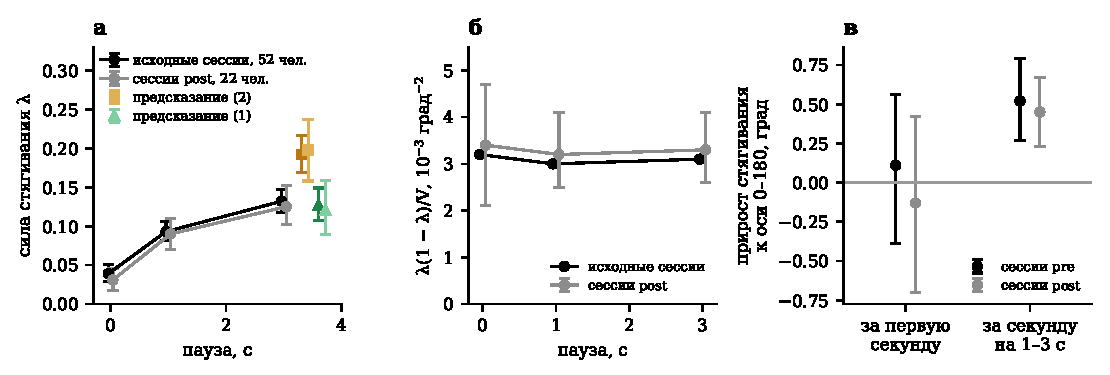
\includegraphics[width=\textwidth]{fig1.pdf}
\caption{(а)~Сила стягивания к диагоналям и два предсказания для паузы 3~с. (б)~Отношение из закона~(\ref{eq:law})
при трёх паузах; для исходных сессий интервалы не считались. (в)~Прирост общего стягивания к оси $0$--$180\gr$ у одних и тех же 22 человек в двух сессиях.}
\end{figure}

\textbf{2.3. Сдвиг в одну сторону} (один период на круг). Все запомненные положения смещены к направлению
$-89\gr$ \ci{-107\gr}{-70\gr} в координатах файла данных; размах общей части при 3~с равен $2,5\gr$. Часть сдвига
($1,3\gr$) есть уже при нулевой паузе. Остальное растёт вслед за неопределённостью: в сессиях \texttt{post}
поздний прирост равен $0,23\gr$ при предсказанных $0,22\gr$, тогда как постоянная скорость давала бы
$1,87\gr$ (разность $-1,64\gr$ \ci{-2,75}{-0,59}).

\textbf{2.4. Поздний дрейф к оси $0$--$180\gr$} (два периода на круг). Общая для людей часть отсутствует при 0~с
и в первую секунду, а на отрезке 1--3~с растёт со скоростью $0,52\gr$/с \ci{0,39}{0,67} в разведке и
$0,45\gr$/с \ci{0,23}{0,67} в сессиях \texttt{post} (рис.~1в). Прирост за первую секунду там равен
$-0,13\gr$ \ci{-0,70}{0,42}; разность раннего и позднего прироста $-0,58\gr$ \ci{-1,16}{-0,01}.
Закону~(\ref{eq:law}) эта составляющая не подчиняется: она должна была бы расти в основном в первую секунду.

\textbf{2.5. Личные поля устойчивы.} У каждого человека свои направление сдвига и ось; они сохраняются через
3--12 месяцев: корреляция личных векторов между сессиями $0,52$ \ci{0,15}{0,77} для одного периода и
$0,69$ \ci{0,51}{0,87} для двух.

\textbf{2.6. Случайный разброс у осей растёт быстрее, чем у диагоналей.} Отношение дисперсий <<у оси / у диагонали>>
в исходных сессиях равно $1,15$, $1,37$ и $1,69$ при паузах 0, 1 и 3~с; в сессиях \texttt{post} его прирост от 0
к 3~с равен $0,35$ \ci{0,05}{0,71}.

\textbf{2.7. Сверка с публикацией.} Влияние предыдущей пробы воспроизводится: у здоровых отталкивание при 0~с
($-0,5\gr$) сменяется притяжением при 3~с ($+2,2\gr$ \ci{1,5}{3,0}); при шизофрении отталкивание сохраняется
при всех паузах (от $-0,8\gr$ до $-1,5\gr$); при энцефалите картина промежуточная.

\section*{3. Замечено после расчёта и не проверено}

\begin{itemize}
\item При шизофрении лишний случайный разброс сосредоточен у осей: при 3~с дисперсия у диагоналей та же, что
у здоровых ($26,7$ и $27,1~\dsq$), а у осей больше ($55,2$ и $37,8~\dsq$).
\item Случайная дисперсия у больных выше уже при 1~с ($22$, $30$ и $34~\dsq$ у здоровых, при шизофрении и при
энцефалите), а скорость её дальнейшего роста одинакова, около $4~\dsq$/с.
\item Константа $V_p$ у больных больше: около $240$, $340$ и $470~\dsq$. Больные стягиваются к диагоналям слабее,
чем следовало бы при их неточности.
\item При шизофрении нет предпочтения оси $0$--$180\gr$ и больше смещение при нулевой паузе
($4,1\gr$ против $2,4\gr$).
\end{itemize}
Больных шизофренией в повторных сессиях нет, поэтому проверить это на тех же данных нельзя.

\section*{4. Не подтвердилось или не решено}

\begin{itemize}
\item \textbf{Привязка личных осей к осям экрана.} В разведке ось лежала близко к $0\gr$ или $90\gr$ у 38 человек
из 52; в сессиях \texttt{post} --- у 13 из 22 при пороге 16.
\item \textbf{Восстановление при энцефалите.} Предсказанный рост отношения $\lambda(1-\lambda)/V$ от первой сессии
ко второй имеет нужный знак, но неотличим от нуля: $+0,0005$ \ci{-0,0003}{0,0011}.
\item \textbf{Связь между людьми.} Корреляция силы стягивания со случайной дисперсией равна $0,14$
\ci{-0,15}{0,41}. Закон~(\ref{eq:law}) выполняется у человека во времени, но не объясняет различий между людьми.
\item \textbf{Закон роста случайной части.} Основная потеря точности ($8$--$17~\dsq$) приходится на первую секунду.
Из-за того что при нулевой паузе памяти нет, отличить диффузию с начальной потерей от насыщения нельзя.
\item \textbf{Сравнение с Gold и соавт. (2020).} Разность наклонов разброса у больных и здоровых равна $-0,03$
\ci{-0,28}{0,22}~град/с; интервал слишком широк, чтобы подтвердить или опровергнуть их эффект $0,16$.
\end{itemize}

\section*{5. Ограничения}

\begin{itemize}
\item Пауз всего три, поэтому о ходе во времени можно судить по двум отрезкам.
\item Данные не различают, возникает ли стягивание в момент ответа или нарастает во время паузы вместе
с неопределённостью. Отвергнут только снос с постоянной скоростью.
\item Неизвестно, где на экране угол $+90\gr$; все направления даны в координатах файла.
\item В сессиях \texttt{post} те же люди, что в исходных. Это проверка устойчивости, а не перенос на новых людей.
\item Взгляд не отслеживался; больные получали лекарства.
\end{itemize}

\section*{6. Первое приближение}

Проверенные закономерности складываются в описание ошибки ответа:
\begin{equation}
\varepsilon=-\lambda(t)\,\delta(\theta)+A_1(t)\sin(\varphi_1-\theta)+A_2(t)\sin 2(\varphi_2-\theta)
+\beta_g(t)\,D(\theta_{\text{пред}}-\theta)+\xi ,\qquad \operatorname{Var}\xi=V(t),
\end{equation}
где $\lambda$ задаётся законом~(\ref{eq:law}); $A_1$ состоит из постоянной части и части, растущей вместе с $V$,
$\varphi_1\approx-89\gr$; общая часть $A_2$ равна нулю до 1~с и затем растёт со скоростью около $0,45$--$0,5\gr$/с
при $\varphi_2\approx0\gr$; $D$ --- нормированная производная гауссианы шириной $0,8$~рад, $\beta_g$ зависит от
группы. Случайная дисперсия составляет около $12~\dsq$ при 0~с, $28$ при 1~с и $37$ при 3~с; после первой секунды она
растёт примерно на $4~\dsq$ в секунду. Это описание ответов, а не модель механизма.

\section*{Источники и материалы}

{\small
Stein H., Barbosa J. и соавт. Reduced serial dependence suggests deficits in synaptic potentiation in anti-NMDAR
encephalitis and schizophrenia. \emph{Nature Communications} 2020; 11: 4250. doi:10.1038/s41467-020-18033-3.
Данные: \texttt{github.com/comptelab/serialNMDA}.

Gold J.\,M. и соавт. Refining the empirical constraints on computational models of spatial working memory in
schizophrenia. \emph{Biol. Psychiatry Cogn. Neurosci. Neuroimaging} 2020; 5(9): 913--922.

Расчёты: скрипты \texttt{wm\_stein.py} -- \texttt{wm\_stein6.py}; каждый содержит проверку метода на искусственных
данных с известным ответом.
}

\end{document}
